\chapter{Resultados}\label{cap4_resultados}

{ Após a exposição dos componentes do ambiente de aprendizado e estrutura das
    implementações do processador, é possível realizar análises quantitativas
    e qualitativas dos resultados obtidos.
}

{ As seções desse capítulo explorarão os resultados da síntese e simulação de
    cada versão, além de apresentar resultados de \textit{benchmarks} sintéticos
    a fim de comparar o desempenho de cada implementação e sua viabilidade de uso.
}

\section{Síntese dos \textit{soft-cores}}
    {
    }
    \begin{longtable}{|l|}
        \caption{Recursos físicos utilizados}\label{table:synth_resources}\\
        \hline
        \hline
        \endfirsthead
        \hline
        \hline
        \endhead
        \hline
    \end{longtable}

\section{Formas de Onda das Simulações}
    {
    }

    \begin{figure}[H]
    \centering
        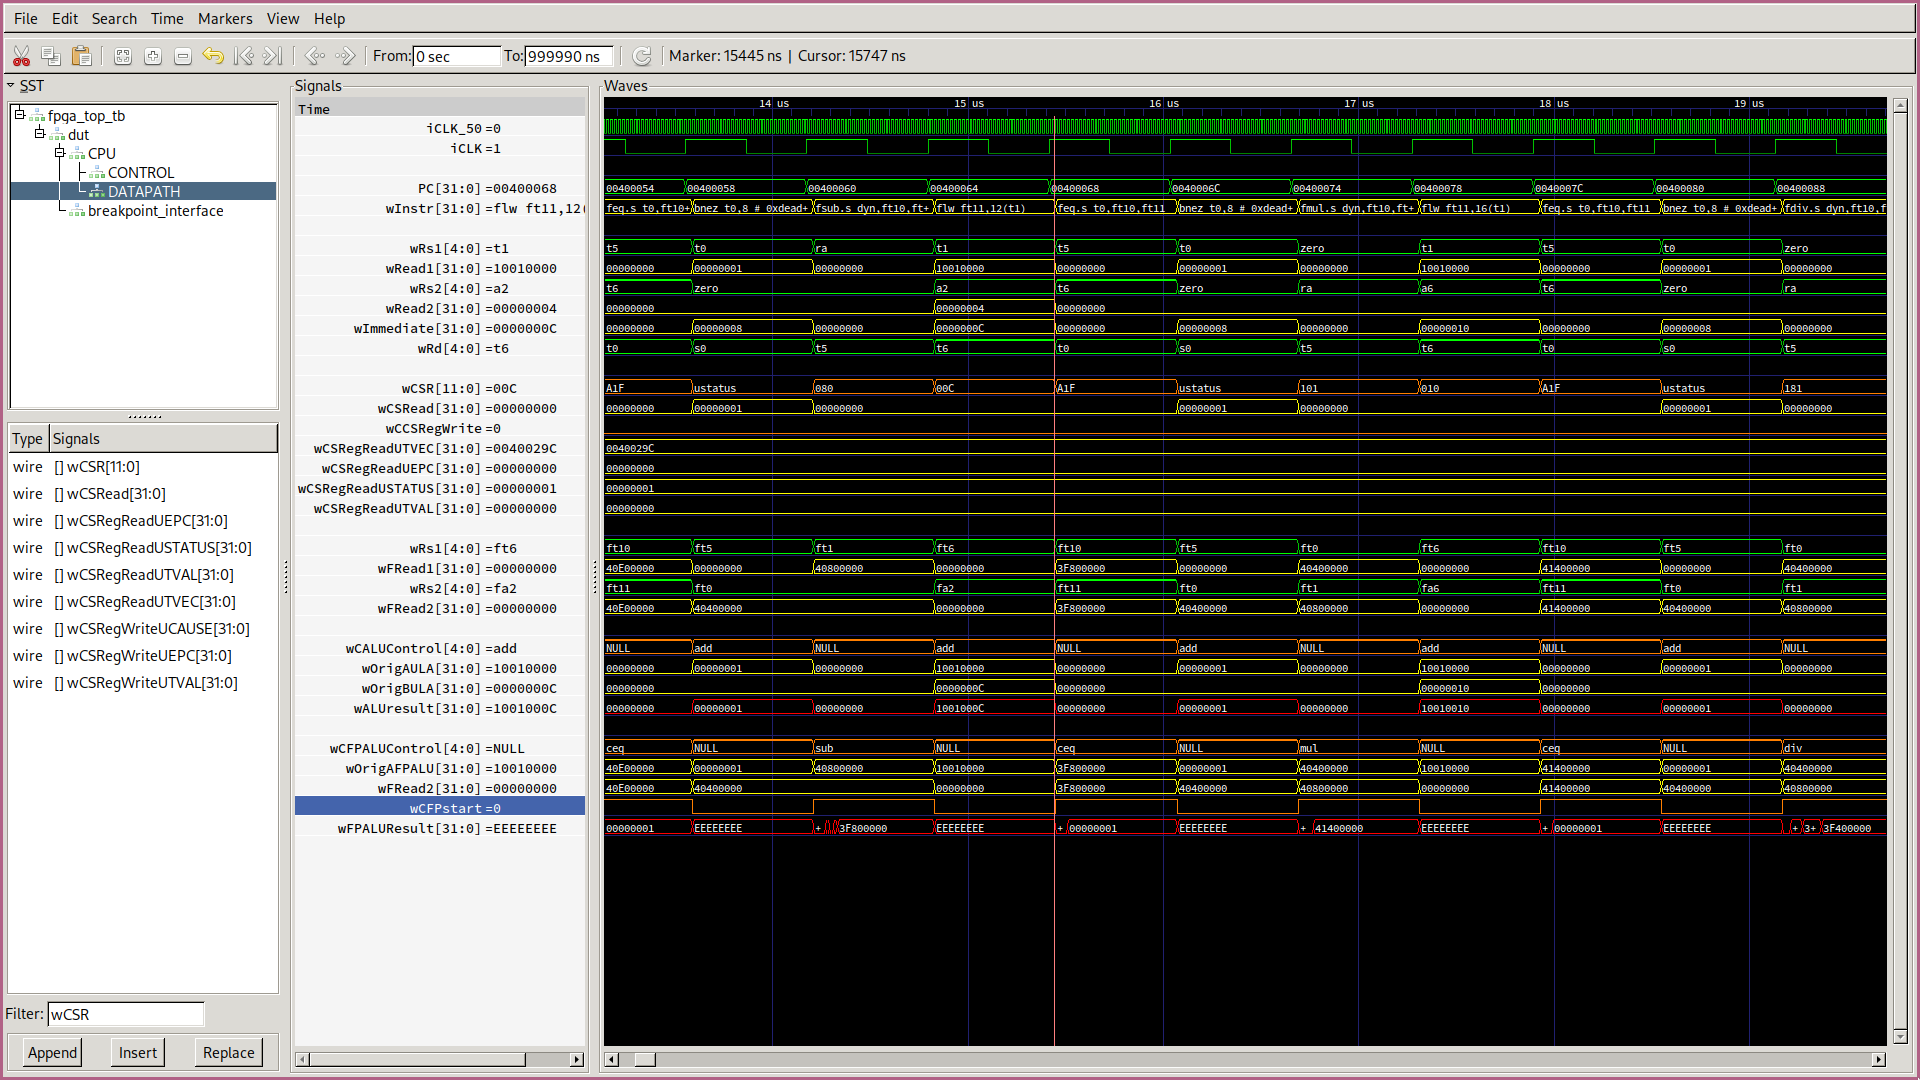
\includegraphics[width=0.9\linewidth]{../images/gtkwave/gtkwave_uni.png}
        \caption{Visualização das formas de onda simuladas do \textit{soft-core} uniciclo}
        \label{fig:gtkwave_uni}
    \end{figure}

    \begin{figure}[H]
    \centering
        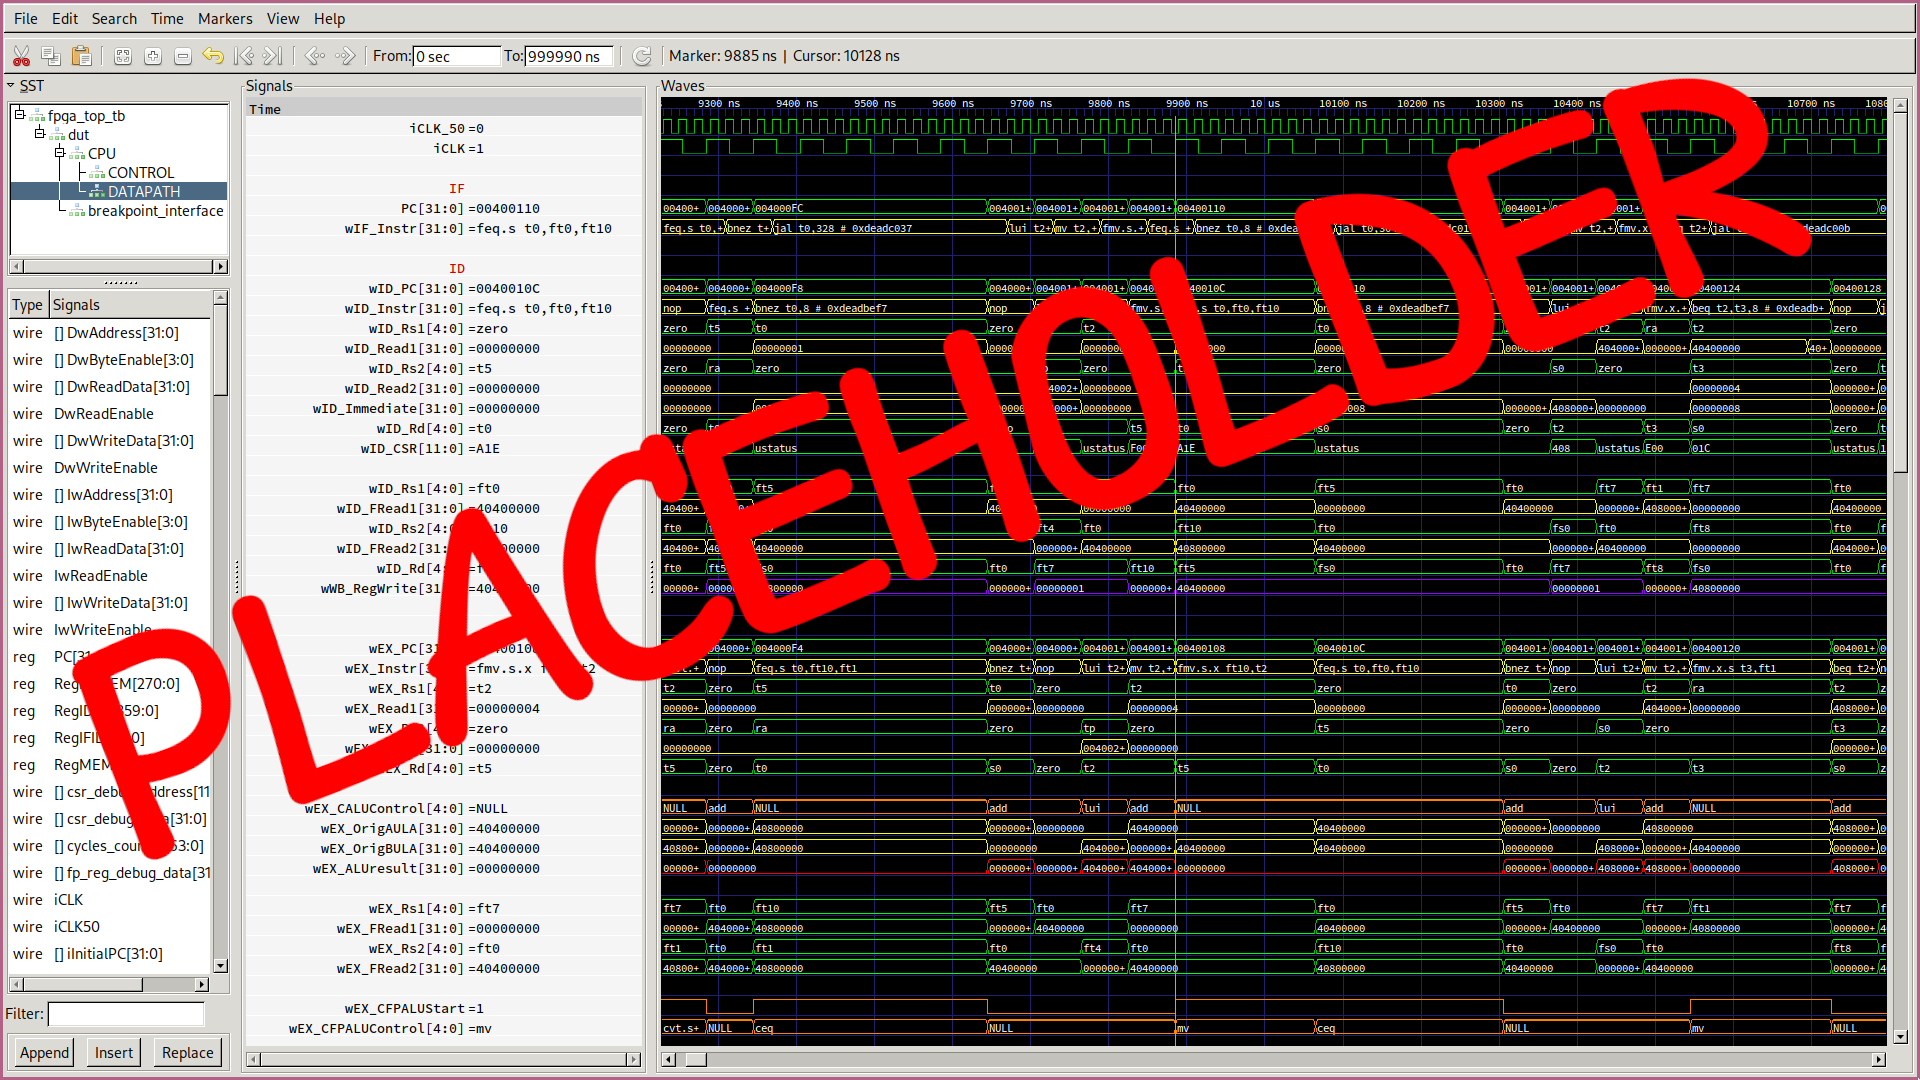
\includegraphics[width=0.9\linewidth]{../images/gtkwave/gtkwave_multi.png}
        \caption{Visualização das formas de onda simuladas do \textit{soft-core} multiciclo}
        \label{fig:gtkwave_multi}
    \end{figure}

    \begin{figure}[H]
    \centering
        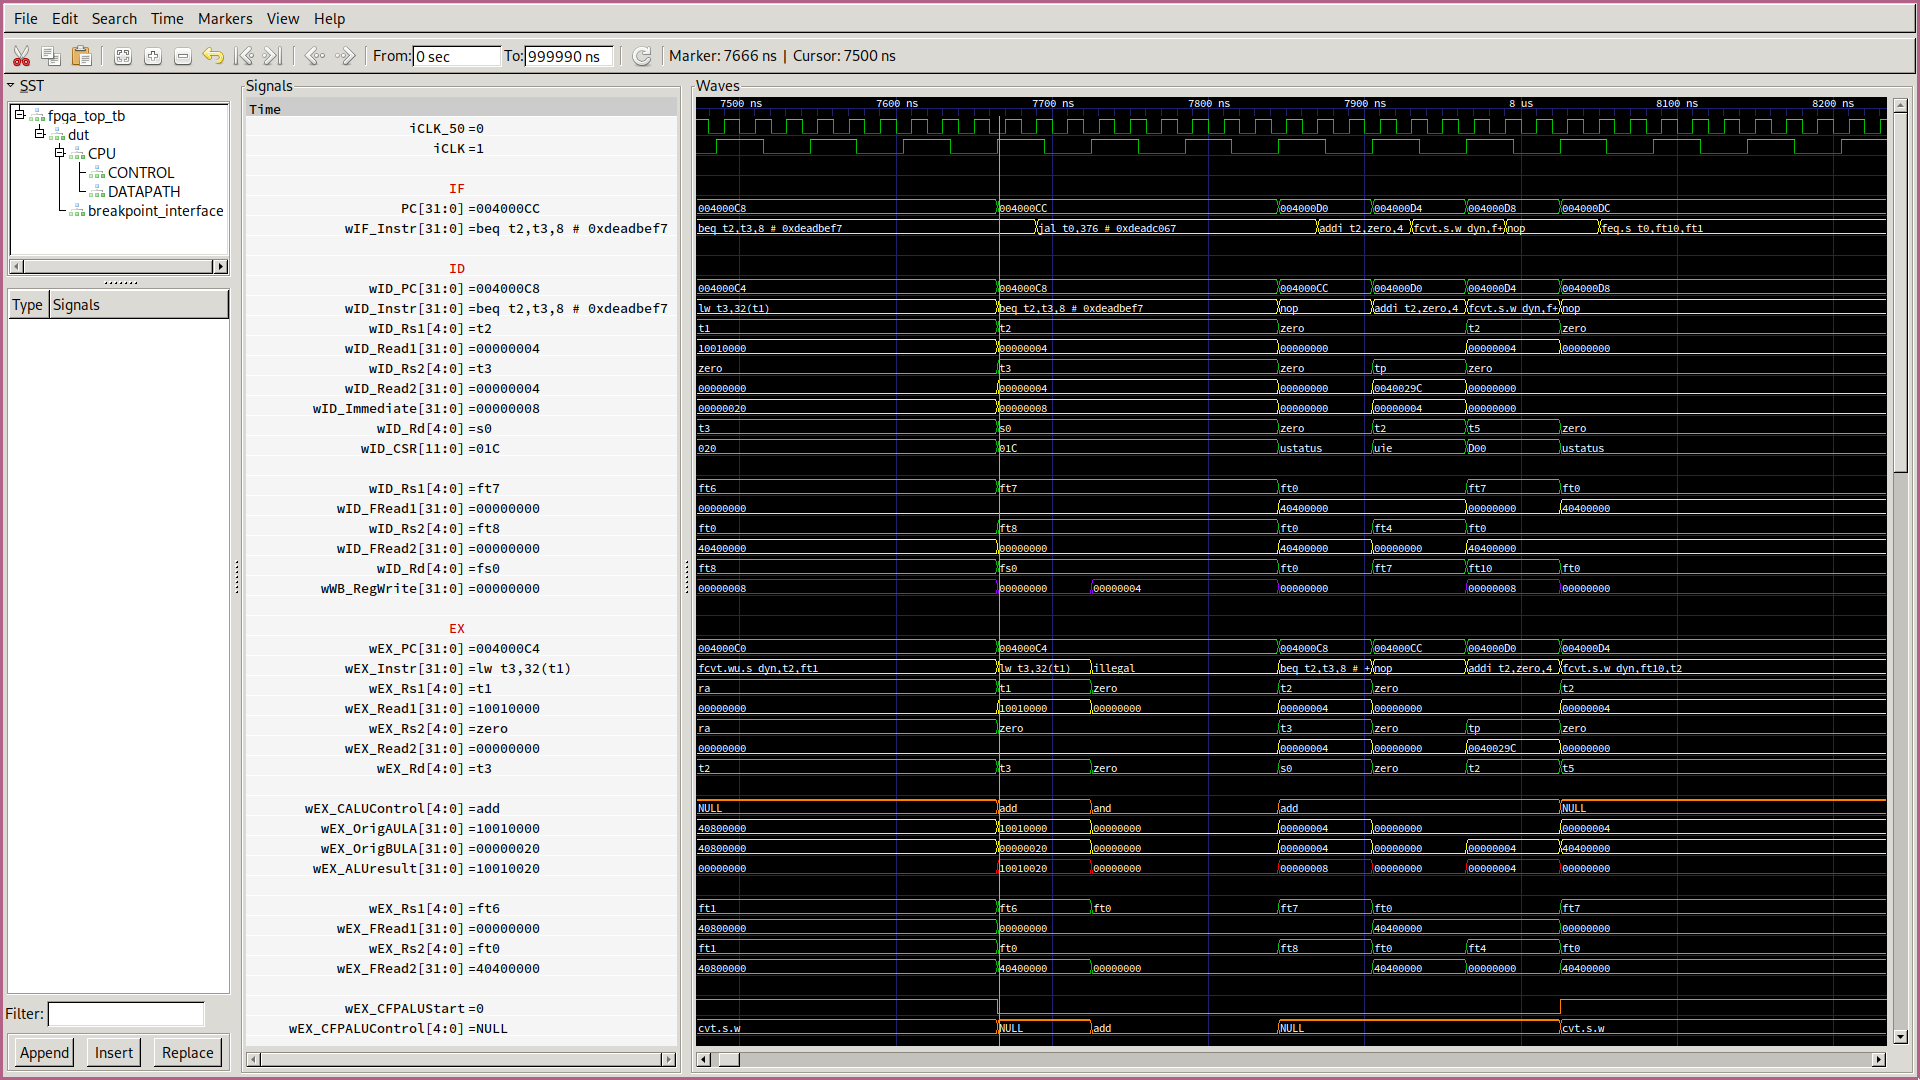
\includegraphics[width=0.9\linewidth]{../images/gtkwave/gtkwave_pipe.png}
        \caption{Visualização das formas de onda simuladas do \textit{soft-core pipeline}}
        \label{fig:gtkwave_pipe}
    \end{figure}

\section{\textit{Benchmarks}}
    {
    }
    \begin{longtable}{|l|}
        \caption{\textit{Benchmark}}\label{table:benchmark}\\
        \hline
        \hline
        \endfirsthead
        \hline
        \hline
        \endhead
        \hline
    \end{longtable}

\section{Observações Finais dos Resultados}
    { Ih, quê isso? Michael Douuuuglaaxxxxx! Nunca mais eu vou dormir, nunca mais
        eu vou dormir...
    } % XXX

    { O próximo capítulo encerrará o presente trabalho fazendo observações
        pertinentes aos resultados obtidos, à viabilidade do uso da plataforma
        desenvolvida para os propósitos desejados e perspectivas futuras,
        tratando de possíveis melhorias e expansão do escopo.
    }

